% !TEX root = ../Dokumentation.tex
\subsection{Objekterkennung}
Die Objekterkennung hat das Ziel die richtigen Objekte zu erkennen und das genaue Positionieren des Fahrzeuges zu ermöglichen. Dabei wird die Containererkennung in zwei Teilaufgaben aufgeteilt: Die \glqq{Objekterkennung grob}\grqq{} ist für die Erkennung der richtigen Objekte mittels Farb- und Formerkennung zuständig. Die \glqq{Objekterkennung präzise}\grqq{} ist für das Positionieren des Fahrzeuges notwendig. Diese zwei Teilaufgaben werden separat angeschaut.
%
\subsubsection{Objekterkennung grob}
Die Aufgabe der \glqq{Objekterkennung grob}\grqq ist es, die aufzuladenden Container, kreuzenden Fahrzeuge und das Entleerungsbecken zu erkennen. Sobald ein solches Objekt erkannt wird, wird der zentrale Controller darüber informiert, damit die Informationen an die \glqq{Objekterkennung}\grqq{} präzise weitergegeben werden können.
\\[0.2cm]
\underline{\textbf{Container}}
\\[0.2cm]
\textbf{Funktionsbeschrieb}\\[0.2cm]
Die Objekterkennung ist zuständig, dass die blauen und Container, welche am Strassenrand stehen, erkannt werden. Wird ein solches Objekt erkannt, wird der Controller darüber informiert, welcher die Informationen anschliessend an den Microcontroller weiterleitet. Das Entleerungsbecken wird nicht mehr, wie in der Konzeptphase geplant, über die Objekterkennung erkannt. Da das Entleerungsbecken weiss ist, würde es bei der Farberkennung zu viele Störobjekte haben. Neu ist die Fahrbahnerkennung dafür verantwortlich.
\\[0.2cm]
Sobald die ersten Bilder mit der Kamera aufgenommen wurden, werden diese laufend aus dem Bilderpool abgefragt und untersucht. Dabei läuft die Erkennung von grünen und blauen Containern parallel ab.
\begin{figure}[H]%Position festigen
\centering
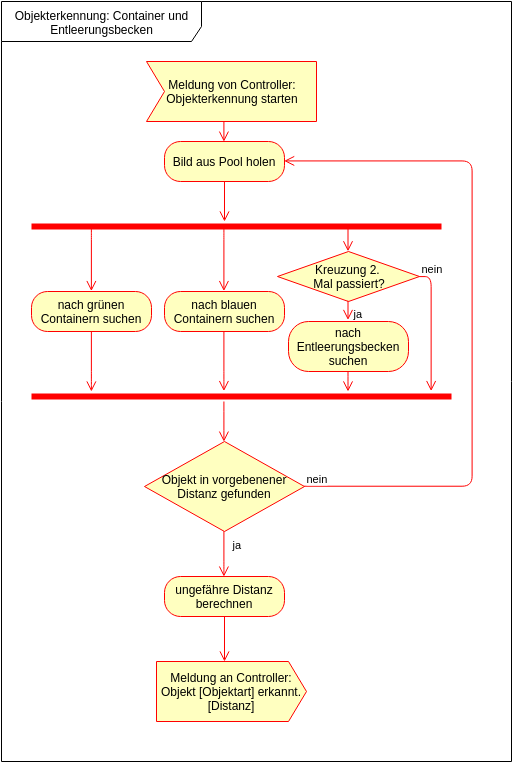
\includegraphics[width=0.6\textwidth]{03_Loesungskonzept/pictures/objekterkennung_containers.png}
\caption{Aktivitätendiagramm Obkjekterkennung: Container}
\label{fig:activityContainer}
\end{figure}
\newpage
Die Erkennung läuft dabei immer gleich ab. Als erstes wird das Bild mit OpenCV nach der entsprechenden Farbe gefiltert. Sprich: Es wird nur nach Grün- und Blautönen gesucht. Anschliessend werden mit Hilfe einer Konturenerkennung störende und falsche Objekte entfernt. Mit störenden Objekten sind Objekte gemeint, welche nicht die Masse eines Containers haben, welcher sich in einem Abstand verbindet, dass er interessant sein könnte. Mit der Höhe dieser Objekte kann dann ausgerechnet werden, wie weit das Objekt  noch entfernt ist. Diese Distanzberechnung liefert nur ein ungefähres Ergebnis. Auf dem Bild wurde eine Meldelinie definiert. Wird diese vom Zentrum des Containers überschritten, wird eine Meldung an den Controller gesendet, welche die Distanz zum Container enthält. Die folgende Darstellung soll die einzelnen Schritte verdeutlichen.
\begin{figure}[H]%Position festigen
\centering
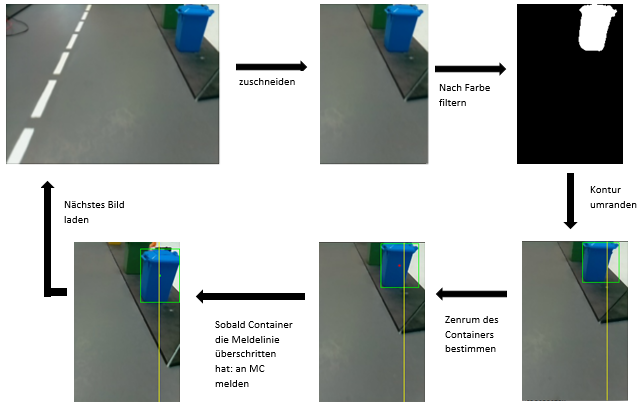
\includegraphics[width=1\textwidth]{03_Loesungskonzept/pictures/uebersicht_object.PNG}
\caption{Ablauf der Obkjekterkennung: Container}
\label{fig:objectDetectionOverview}
\end{figure}
Um den Container zu identifizieren werden die Positionen der Zentren analysiert. Falls sich ein Zentrum um mehr als 10 Pixel seit dem letzten Bild verschoben hat, handelt es sich um einen neuen Container.

Die ungefähre Distanz des Containers wird anhand von Referenzgrössen bestimmt.

\[
Distanz = \frac{Referenzpixelhöhe\cdot Referenzdistanz}{Pixelhöhe}
\]
\begin{figure}[H]%Position festigen
\centering
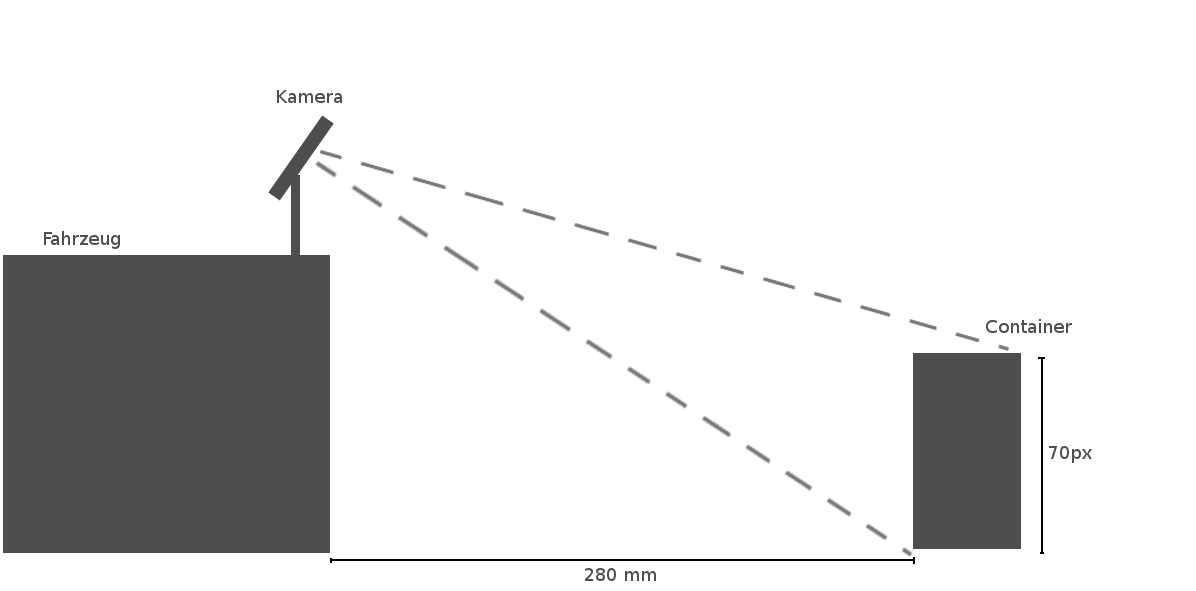
\includegraphics[width=1\textwidth]{03_Loesungskonzept/pictures/distance_reference.png}
\caption{Distanzbemessung}
\label{fig:distanceCalculation}
\end{figure}
\\[0.2cm]
\textbf{Vergleich Konzept und Umsetzung}\\[0.2cm]
Wie bereits erwähnt, ist die Erkennung des Entleerungsbecken nicht mehr Teil der Objekterkennung. Auch der Zeitpunkt für die Meldung an den Container musste überdenkt werden, da der Controller und somit auch das Microcontroller-Board mehrmals über denselben Container informiert worden wäre. Dazu wurde der Meldebalken eingefügt.

\underline{\textbf{Rechtsvortritt}}\\[0.2cm]
Sobald das Fahrzeug an der Kreuzung angelangt ist, wird dies der Objekterkennung mitgeteilt und die Kamera wird gedreht. Um nun festzustellen werden im aktuellen Bild alle gefundenen Kanten gesucht. Diese Anzahl Kanten wird mit einer Referenzanzahl verglichen. Ist die Anzahl massiv grösser als die Referenzanzahl, wird davon ausgegangen, dass sich ein Fahrzeug an der Kreuzung befindet.\\[0.2cm]
\textbf{Vergleich Konzept und Umsetzung}\\[0.2cm]
In Pren1 wurde die Rechtsvortritterkennung aufwändiger geplant. Die Fahrbahnerkennung sollte die Kreuzung erkennen und anschliessend Koordinaten des Bildes an die Objekterkennung senden. Diese Koordinaten waren die Eckpunkte der Fahrbahn, welche sich von rechts nähert. Anschliessen wäre der Bereich untersucht worden, um festzulegen, ob sich ein Fahrzeug darauf befindet oder nicht. Da die Kamera nun jedoch so positioniert werden musste, dass die Fahrbahn möglichst nahe am Fahrzeug schon erkennt werden kann, gehen Informationen in der Ferne verloren. Wobei auch der abzusuchende Teil der Strecke kleiner wurde.

\subsubsection{Objekterkennung präzise}
\underline{\textbf{Containererkennung}}\\[0.2cm]
Das präzise Stoppen beim Container wird vom Mikrocontrollerboard gesteuert. Der Aufladevorgang wird eingeleitet, wenn das Freedomboard den Befehl StA d Wert bekommt. Dabei gibt der Wert den ungefähren Abstand zum aufzuladenden Container vor. Der Mikrocontroller drosselt daraufhin die Fahrgeschwindigkeit auf 100mm/s und berechnet die Zeitdauer bis das Fahrzeug den Container ungefähr erreicht. Kurz bevor dies der Fall ist, beginnt das Freedombaord den Infrarotsensor auszuwerten. Detektiert der Infrarotsensor nun ein Objekt über eine längere Zeit, ist ein Container gefunden. Sobald das der Infrarotsensor nun kein Objekt mehr detektiert, stoppt das Fahrzeug. Durch die richtige Platzierung des Infrarotsensors steht der Greifer nun exakt über dem aufzuladenden Container.\\[0.2cm]
\textbf{Vergleich Konzept und Umsetzung}\\[0.2cm]
Das Konzept mit dem präzisen anhalten über den Infrarotsensor hat sich im Pren2 nicht geändert.
%
\underline{\textbf{Entleerungsbecken Erkennung}} \\[0.2cm]
Die Erkennung des Entleerungsbecken wurde sehr simpel gelöst. Sobald das Fahrzeug erkennt das es im Zielfels steht, ist bereits klar wo das Entleerungsbecken steht. Somit ist eine extra Erkennung des Entleerungsbecken nicht mehr notwendig.\\[0.2cm]
\textbf{Vergleich Konzept und Umsetzung}\\[0.2cm]
Das Konzept zur Detektion des Entleerungsbecken konnte vereinfacht werden. Im Pren1 wurde angenommen, dass man das Entleerungsbecken extra erkennen muss. Es hat sich jetzt jedoch im Pren2 herausgestellt, dass die Fahrpräzision so gut ist, das es keine extra Detektion braucht. (Es muss nicht extra nahe an das Becken herangefahren werden.)

\underline{\textbf{Rechtsvortritt}}\\[0.2cm]
Damit Kollisionen mit anderen Fahrzeugen vermieden werden können, wurde ein Ultraschallsensor eingebaut. Dieser misst über kurze Ultraschallpulse die Distanz zum nächsten Objekt. Die Ansteuerung und Auswertung wurde auf dem Mikrocontrollerboard realisiert. Die Grundlage der Implementierung basiert auf diesem Tutorial: mcuoneclipse.com. Jedoch wurde dieser Code noch effizienter gestaltet.\\[0.2cm]
\textbf{Vergleich Konzept und Umsetzung}\\[0.2cm]
Die Ansteuerung des Ultraschallsensor konnte bereits im Pren1 als Funktionsmuster erfolgreich getestet werden. Daher musste im Pren2 nichts am bestehenden Konzept geändert werden.